\documentclass{article}
\usepackage{amsmath}
\usepackage{graphicx}
\usepackage{geometry}
\usepackage{listings}
\geometry{a4paper, margin=1in}

\begin{document}

\section*{Question 6: Adam Optimizer Implementation}

I have implemented the Adam optimizer from scratch using NumPy and applied it to the logistic regression model from Assignment 1.

\subsection*{Implementation}
The Adam optimizer logic is encapsulated in an `Adam` class. It maintains moving averages of the gradients (\(m\)) and the squared gradients (\(v\)), which are updated at each step. The parameters are then updated based on these bias-corrected estimates. The full implementation can be found in the accompanying `question6.py` file.

\subsection*{Comparison with SGD}
I compared the convergence speed of the Adam optimizer against the standard SGD optimizer. For this comparison, I used the following learning rates:
\begin{itemize}
    \item \textbf{Adam}: \(10^{-2}\)
    \item \textbf{SGD}: \(10^{-4}\)
\end{itemize}
The plot below shows the training loss over 1000 epochs for both optimizers on a synthetic dataset.

\begin{figure}[h!]
\centering
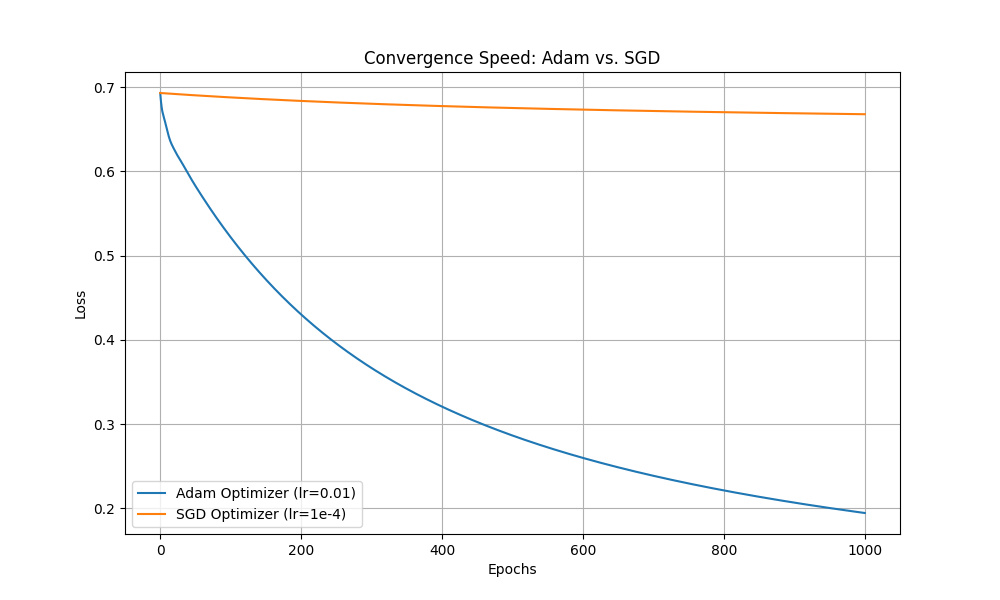
\includegraphics[width=0.8\textwidth]{convergence_comparison.png}
\caption{Convergence speed comparison between Adam and SGD.}
\label{fig:convergence}
\end{figure}

As seen in the figure, the Adam optimizer converges significantly faster and achieves a lower loss value compared to SGD with the given learning rates. Adam's adaptive learning rate mechanism allows it to make larger, more effective updates in the initial stages of training, leading to quicker convergence.

\end{document}
